\documentclass[11pt,a4paper]{article}
\usepackage[utf8]{inputenc}
\usepackage[T1]{fontenc}
\usepackage{geometry}
\usepackage{graphicx}
\usepackage{xcolor}
\usepackage{longtable}
\usepackage{booktabs}
\usepackage{array}
\usepackage{multirow}
\usepackage{tikz}
\usepackage{pgfplots}
\usepackage{fancyhdr}
\usepackage{titlesec}
\usepackage{enumitem}
\usepackage{hyperref}
\usepackage{amsmath}

\geometry{left=2cm,right=2cm,top=2.5cm,bottom=2.5cm}
\pgfplotsset{compat=1.18}

% Colors
\definecolor{primaryblue}{RGB}{0,82,204}
\definecolor{secondaryblue}{RGB}{0,102,255}
\definecolor{accentpink}{RGB}{255,51,102}

% Header and Footer
\pagestyle{fancy}
\fancyhf{}
\fancyhead[L]{\textcolor{primaryblue}{\textbf{SavoyConnect Project Timeline}}}
\fancyhead[R]{\textcolor{gray}{November 2025}}
\fancyfoot[C]{\thepage}
\renewcommand{\headrulewidth}{2pt}
\renewcommand{\headrule}{\hbox to\headwidth{\color{primaryblue}\leaders\hrule height \headrulewidth\hfill}}

% Title formatting
\titleformat{\section}
  {\Large\bfseries\color{primaryblue}}
  {\thesection}{1em}{}[\titlerule]

\titleformat{\subsection}
  {\large\bfseries\color{secondaryblue}}
  {\thesubsection}{1em}{}

\hypersetup{
    colorlinks=true,
    linkcolor=primaryblue,
    urlcolor=secondaryblue,
    citecolor=accentpink
}

\begin{document}

% Title Page
\begin{titlepage}
    \centering
    \vspace*{2cm}
    
    {\Huge\bfseries\color{primaryblue} SavoyConnect\par}
    \vspace{0.5cm}
    {\LARGE\color{accentpink} Project Timeline \& Resource Estimation\par}
    \vspace{2cm}
    
    {\Large\textbf{Single Developer Implementation Plan}\par}
    \vspace{1cm}
    
    
\begin{tikzpicture}
        \draw[primaryblue, line width=2pt] (0,0) -- (12,0);
    \end{tikzpicture}
    
    \vspace{2cm}
    
    \begin{tabular}{ll}
        \textbf{Tech Stack:} & MySQL + Laravel + Flutter + Next.js \\
        \textbf{Project Type:} & Ice Cream Ordering \& Delivery Platform \\
        \textbf{Estimated Duration:} & 23.2 months \\
        \textbf{Total Man-Hours:} & 3710 hours \\
        \textbf{Document Date:} & November 3, 2025 \\
    \end{tabular}
    
    \vfill
    
    {\large Prepared for: Management Review \& Planning\par}
    
\end{titlepage}

\tableofcontents
\newpage

\section{Executive Summary}

\subsection{Project Overview}
SavoyConnect is a comprehensive ice cream ordering and delivery platform featuring custom box creation, loyalty rewards, social features, and real-time order tracking. This document provides a detailed timeline and resource estimation for a \textbf{single developer} implementing the entire system.

\subsection{Key Metrics}

\begin{table}[h]
\centering
\begin{tabular}{|l|r|}
\hline
\rowcolor{primaryblue!20}
\textbf{Metric} & \textbf{Value} \\
\hline
Total Man-Hours & 3710 hours \\
\hline
Full-Time Equivalent & 23.2 months (160 hrs/month) \\
\hline
Working Days (8 hrs/day) & 464 days \\
\hline
Working Weeks (40 hrs/week) & 93 weeks \\
\hline
Calendar Months (Estimate) & 23.2 months \\
\hline
Development Phases & 7 phases \\
\hline
\end{tabular}
\caption{Project Resource Summary}
\end{table}

\subsection{Technology Stack}

\begin{itemize}[leftmargin=2cm]
    \item \textbf{Backend:} Laravel (PHP) - RESTful API, Authentication, Business Logic
    \item \textbf{Database:} MySQL - Relational Database Management
    \item \textbf{Mobile App:} Flutter - Cross-platform (iOS \& Android)
    \item \textbf{Web Application:} Next.js (React) - Server-Side Rendering
    \item \textbf{Additional:} Payment Gateway, Push Notifications, Real-time Tracking
\end{itemize}

\subsection{Assumptions}

\begin{enumerate}
    \item Single developer working full-time (8 hours/day, 40 hours/week)
    \item Developer proficient in all required technologies
    \item No major scope changes during development
    \item Third-party services (payment gateway, hosting) readily available
    \item Standard complexity for integrations
\end{enumerate}

\newpage

\section{Phase Breakdown}


\subsection{Phase 1: Planning & Design}

\textbf{Duration:} 290 hours (7.2 weeks at 40 hrs/week)

\begin{longtable}{|p{8cm}|r|r|}
\hline
\rowcolor{blue!30}
\textbf{Task} & \textbf{Hours} & \textbf{Days (8h)} \\
\hline
\endfirsthead

\hline
\rowcolor{blue!30}
\textbf{Task} & \textbf{Hours} & \textbf{Days (8h)} \\
\hline
\endhead

Requirements Documentation & 40 & 5.0 \\
\hline
Database Schema Design & 60 & 7.5 \\
\hline
API Specifications & 50 & 6.2 \\
\hline
UI/UX Refinement & 80 & 10.0 \\
\hline
Architecture Documentation & 40 & 5.0 \\
\hline
Sprint Planning & 20 & 2.5 \\
\hline
\rowcolor{gray!20}
\textbf{Phase 1 Total} & \textbf{290} & \textbf{36.2} \\
\hline
\caption{Phase 1 Task Breakdown}
\end{longtable}


\subsection{Phase 2: Backend Development (Laravel + MySQL)}

\textbf{Duration:} 780 hours (19.5 weeks at 40 hrs/week)

\begin{longtable}{|p{8cm}|r|r|}
\hline
\rowcolor{red!30}
\textbf{Task} & \textbf{Hours} & \textbf{Days (8h)} \\
\hline
\endfirsthead

\hline
\rowcolor{red!30}
\textbf{Task} & \textbf{Hours} & \textbf{Days (8h)} \\
\hline
\endhead

Database Setup & Migrations & 60 & 7.5 \\
\hline
Authentication & Authorization System & 80 & 10.0 \\
\hline
User Management APIs & 60 & 7.5 \\
\hline
Product Catalog APIs & 80 & 10.0 \\
\hline
Order Management System & 120 & 15.0 \\
\hline
Payment Gateway Integration & 100 & 12.5 \\
\hline
Delivery Management System & 80 & 10.0 \\
\hline
Admin Panel APIs & 100 & 12.5 \\
\hline
Loyalty Points Calculation Engine & 60 & 7.5 \\
\hline
Notification Service Setup & 40 & 5.0 \\
\hline
\rowcolor{gray!20}
\textbf{Phase 2 Total} & \textbf{780} & \textbf{97.5} \\
\hline
\caption{Phase 2 Task Breakdown}
\end{longtable}


\subsection{Phase 3: Mobile App Development (Flutter)}

\textbf{Duration:} 860 hours (21.5 weeks at 40 hrs/week)

\begin{longtable}{|p{8cm}|r|r|}
\hline
\rowcolor{green!30}
\textbf{Task} & \textbf{Hours} & \textbf{Days (8h)} \\
\hline
\endfirsthead

\hline
\rowcolor{green!30}
\textbf{Task} & \textbf{Hours} & \textbf{Days (8h)} \\
\hline
\endhead

Flutter Project Setup & Architecture & 40 & 5.0 \\
\hline
Authentication Screens & 60 & 7.5 \\
\hline
Home Feed & Navigation & 80 & 10.0 \\
\hline
Product Browsing & Search & 100 & 12.5 \\
\hline
Custom Box Builder Interface & 120 & 15.0 \\
\hline
Shopping Cart & Checkout & 80 & 10.0 \\
\hline
Payment Integration & 80 & 10.0 \\
\hline
Order Tracking Interface & 60 & 7.5 \\
\hline
User Profile & Wallet & 60 & 7.5 \\
\hline
Loyalty Rewards Interface & 60 & 7.5 \\
\hline
Push Notification Setup & 40 & 5.0 \\
\hline
Recipe Sharing Features & 80 & 10.0 \\
\hline
\rowcolor{gray!20}
\textbf{Phase 3 Total} & \textbf{860} & \textbf{107.5} \\
\hline
\caption{Phase 3 Task Breakdown}
\end{longtable}


\subsection{Phase 4: Web Application Development (Next.js)}

\textbf{Duration:} 730 hours (18.2 weeks at 40 hrs/week)

\begin{longtable}{|p{8cm}|r|r|}
\hline
\rowcolor{orange!30}
\textbf{Task} & \textbf{Hours} & \textbf{Days (8h)} \\
\hline
\endfirsthead

\hline
\rowcolor{orange!30}
\textbf{Task} & \textbf{Hours} & \textbf{Days (8h)} \\
\hline
\endhead

Next.js Setup with SSR Configuration & 40 & 5.0 \\
\hline
Authentication Pages & 50 & 6.2 \\
\hline
Responsive Home & Navigation & 60 & 7.5 \\
\hline
Product Catalog with Filtering & 80 & 10.0 \\
\hline
Custom Box Creator & 100 & 12.5 \\
\hline
Checkout Flow & 80 & 10.0 \\
\hline
User Dashboard & 60 & 7.5 \\
\hline
Order Management Interface & 60 & 7.5 \\
\hline
Admin Dashboard & 120 & 15.0 \\
\hline
Analytics & Reporting Pages & 80 & 10.0 \\
\hline
\rowcolor{gray!20}
\textbf{Phase 4 Total} & \textbf{730} & \textbf{91.2} \\
\hline
\caption{Phase 4 Task Breakdown}
\end{longtable}


\subsection{Phase 5: Integration & Testing}

\textbf{Duration:} 540 hours (13.5 weeks at 40 hrs/week)

\begin{longtable}{|p{8cm}|r|r|}
\hline
\rowcolor{purple!30}
\textbf{Task} & \textbf{Hours} & \textbf{Days (8h)} \\
\hline
\endfirsthead

\hline
\rowcolor{purple!30}
\textbf{Task} & \textbf{Hours} & \textbf{Days (8h)} \\
\hline
\endhead

API Integration Testing & 80 & 10.0 \\
\hline
Cross-platform Testing (iOS, Android, Web) & 100 & 12.5 \\
\hline
Payment Gateway Testing & 60 & 7.5 \\
\hline
End-to-End User Journey Testing & 80 & 10.0 \\
\hline
Performance Optimization & 60 & 7.5 \\
\hline
Security Audit & 40 & 5.0 \\
\hline
Bug Fixes & Refinements & 120 & 15.0 \\
\hline
\rowcolor{gray!20}
\textbf{Phase 5 Total} & \textbf{540} & \textbf{67.5} \\
\hline
\caption{Phase 5 Task Breakdown}
\end{longtable}


\subsection{Phase 6: Deployment & Launch}

\textbf{Duration:} 270 hours (6.8 weeks at 40 hrs/week)

\begin{longtable}{|p{8cm}|r|r|}
\hline
\rowcolor{cyan!30}
\textbf{Task} & \textbf{Hours} & \textbf{Days (8h)} \\
\hline
\endfirsthead

\hline
\rowcolor{cyan!30}
\textbf{Task} & \textbf{Hours} & \textbf{Days (8h)} \\
\hline
\endhead

Server Setup & Configuration & 40 & 5.0 \\
\hline
Database Migration to Production & 30 & 3.8 \\
\hline
App Store Submissions (iOS & Android) & 40 & 5.0 \\
\hline
Web Hosting & CDN Setup & 30 & 3.8 \\
\hline
Beta Testing with Real Users & 60 & 7.5 \\
\hline
Launch Preparation & Marketing & 30 & 3.8 \\
\hline
Documentation & User Guides & 40 & 5.0 \\
\hline
\rowcolor{gray!20}
\textbf{Phase 6 Total} & \textbf{270} & \textbf{33.8} \\
\hline
\caption{Phase 6 Task Breakdown}
\end{longtable}


\subsection{Phase 7: Post-Launch Support & Monitoring}

\textbf{Duration:} 240 hours (6.0 weeks at 40 hrs/week)

\begin{longtable}{|p{8cm}|r|r|}
\hline
\rowcolor{yellow!30}
\textbf{Task} & \textbf{Hours} & \textbf{Days (8h)} \\
\hline
\endfirsthead

\hline
\rowcolor{yellow!30}
\textbf{Task} & \textbf{Hours} & \textbf{Days (8h)} \\
\hline
\endhead

Bug Monitoring & Critical Fixes & 80 & 10.0 \\
\hline
User Feedback Collection & Analysis & 40 & 5.0 \\
\hline
Performance Monitoring & Optimization & 40 & 5.0 \\
\hline
Minor Feature Enhancements & 80 & 10.0 \\
\hline
\rowcolor{gray!20}
\textbf{Phase 7 Total} & \textbf{240} & \textbf{30.0} \\
\hline
\caption{Phase 7 Task Breakdown}
\end{longtable}


\newpage

\section{Visual Timeline}

\subsection{Man-Hours Distribution by Phase}

\begin{center}
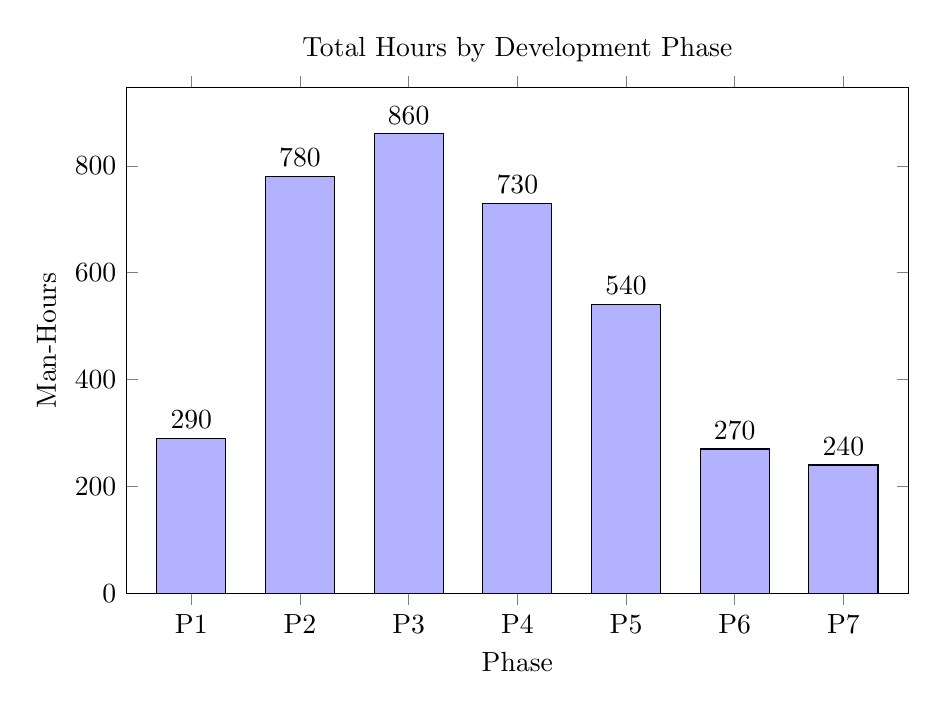
\begin{tikzpicture}
    \begin{axis}[
        ybar,
        bar width=25pt,
        width=0.95\textwidth,
        height=8cm,
        ylabel={Man-Hours},
        symbolic x coords={P1,P2,P3,P4,P5,P6,P7},
        xtick=data,
        nodes near coords,
        nodes near coords align={vertical},
        ymin=0,
        legend style={at={(0.5,-0.15)}, anchor=north,legend columns=-1},
        xlabel={Phase},
        title={Total Hours by Development Phase}
    ]
    \addplot[fill=blue!30] coordinates {
        (P1,290)
        (P2,780)
        (P3,860)
        (P4,730)
        (P5,540)
        (P6,270)
        (P7,240)
    };
    \end{axis}
\end{tikzpicture}
\end{center}

\subsection{Cumulative Progress Chart}

\begin{center}
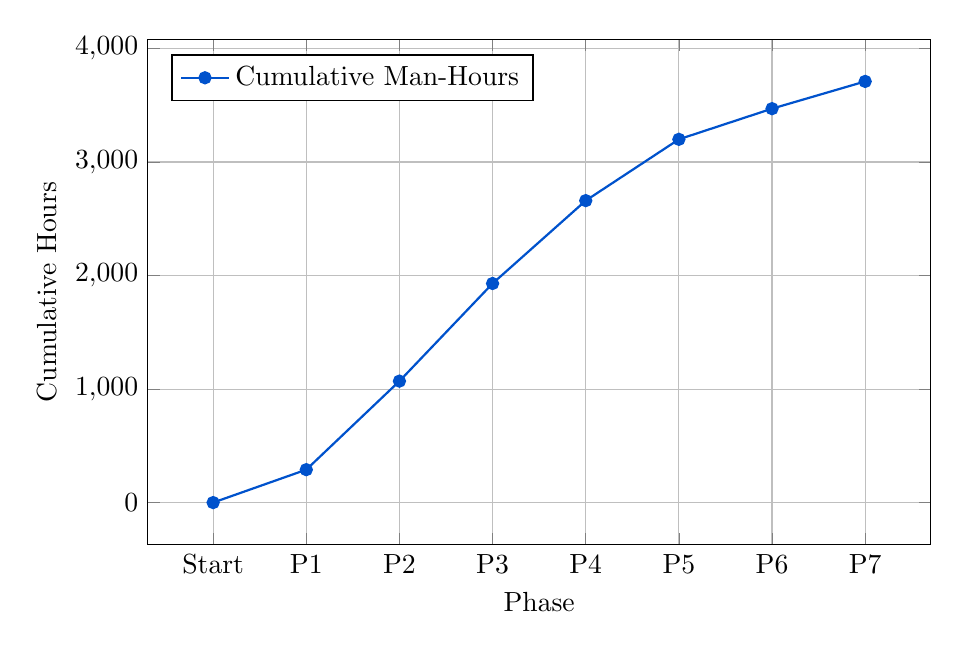
\begin{tikzpicture}
    \begin{axis}[
        width=0.95\textwidth,
        height=8cm,
        xlabel={Phase},
        ylabel={Cumulative Hours},
        symbolic x coords={Start,P1,P2,P3,P4,P5,P6,P7},
        xtick=data,
        legend pos=north west,
        grid=major
    ]
    \addplot[
        color=primaryblue,
        mark=*,
        thick
    ] coordinates {
        (Start,0)
        (P1,290)
        (P2,1070)
        (P3,1930)
        (P4,2660)
        (P5,3200)
        (P6,3470)
        (P7,3710)
    };
    \legend{Cumulative Man-Hours}
    \end{axis}
\end{tikzpicture}
\end{center}


\newpage

\section{Sequential Timeline (Gantt View)}

\subsection{Phase Schedule (Single Developer)}

Assuming continuous full-time work (40 hours/week), here is the sequential timeline:

\begin{longtable}{|l|r|r|r|r|}
\hline
\rowcolor{gray!30}
\textbf{Phase} & \textbf{Hours} & \textbf{Weeks} & \textbf{Start Week} & \textbf{End Week} \\
\hline
\endfirsthead

\hline
\rowcolor{gray!30}
\textbf{Phase} & \textbf{Hours} & \textbf{Weeks} & \textbf{Start Week} & \textbf{End Week} \\
\hline
\endhead

Phase 1 & 290 & 7.2 & 1 & 7.2 \\
\hline
Phase 2 & 780 & 19.5 & 8.2 & 26.7 \\
\hline
Phase 3 & 860 & 21.5 & 27.7 & 48.2 \\
\hline
Phase 4 & 730 & 18.2 & 49.2 & 66.4 \\
\hline
Phase 5 & 540 & 13.5 & 67.4 & 79.9 \\
\hline
Phase 6 & 270 & 6.8 & 80.9 & 86.7 \\
\hline
Phase 7 & 240 & 6.0 & 87.7 & 92.7 \\
\hline
\rowcolor{primaryblue!20}
\textbf{TOTAL} & \textbf{3710} & \textbf{92.8} & \textbf{1} & \textbf{92.7} \\
\hline
\caption{Sequential Phase Timeline}
\end{longtable}


\newpage

\section{Risk Assessment \& Mitigation}

\subsection{Technical Risks}

\begin{table}[h]
\centering
\begin{tabular}{|p{4cm}|p{3cm}|p{6cm}|}
\hline
\rowcolor{red!20}
\textbf{Risk} & \textbf{Probability} & \textbf{Mitigation Strategy} \\
\hline
Payment Gateway Integration Issues & Medium & Use well-documented gateways (Stripe), allocate buffer time \\
\hline
Cross-platform Compatibility & Medium & Regular testing on iOS \& Android devices, use Flutter best practices \\
\hline
Performance Issues & Low & Implement caching, optimize database queries, use CDN \\
\hline
Security Vulnerabilities & Medium & Regular security audits, follow OWASP guidelines, use Laravel security features \\
\hline
Scope Creep & High & Strict scope control, change request process, MVP-first approach \\
\hline
\end{tabular}
\caption{Risk Assessment Matrix}
\end{table}

\subsection{Resource Risks}

\begin{itemize}
    \item \textbf{Single Point of Failure:} One developer means no backup. Mitigation: Good documentation, version control, regular backups.
    \item \textbf{Skill Gaps:} Developer may need learning time for specific technologies. Buffer time included in estimates.
    \item \textbf{Burnout:} Long solo project can lead to fatigue. Recommendation: Regular breaks, realistic scheduling.
\end{itemize}

\subsection{Timeline Risks}

\begin{itemize}
    \item \textbf{Underestimation:} Tasks may take longer than estimated (+20-30\% buffer recommended).
    \item \textbf{Unforeseen Challenges:} Technical blockers, API changes, third-party service issues.
    \item \textbf{Testing Overhead:} Manual testing across platforms is time-consuming.
\end{itemize}

\section{Recommendations}

\subsection{For Management}

\begin{enumerate}
    \item \textbf{Add 25-30\% Buffer:} Realistic timeline should account for unknowns (4638-4823 hours total).
    \item \textbf{Consider MVP Approach:} Launch core features first, iterate with user feedback.
    \item \textbf{Quality Assurance:} Budget for external QA or beta testing to reduce developer testing burden.
    \item \textbf{Infrastructure Ready:} Ensure servers, domains, payment accounts are set up before deployment phase.
\end{enumerate}

\subsection{For Developer}

\begin{enumerate}
    \item \textbf{Prioritize Core Features:} Authentication, ordering, payment must be rock-solid.
    \item \textbf{Use Boilerplates:} Laravel starter kits, Flutter templates can save 20-30 hours.
    \item \textbf{Automated Testing:} Write unit tests for critical backend logic (saves debugging time).
    \item \textbf{Version Control:} Commit regularly, use branches for features.
    \item \textbf{Documentation:} Document as you go, especially API endpoints and data models.
\end{enumerate}

\subsection{Success Metrics}

\begin{itemize}
    \item Complete each phase within 10\% of estimated hours
    \item Zero critical bugs in production launch
    \item App store approval on first submission
    \item 95\%+ uptime in first month post-launch
    \item Positive user feedback on core features
\end{itemize}

\newpage

\section{Appendix}

\subsection{A. Technology Justification}

\textbf{Laravel (Backend):}
\begin{itemize}
    \item Rapid development with built-in auth, ORM, validation
    \item Large ecosystem and community support
    \item Estimated time savings: 50+ hours vs. building from scratch
\end{itemize}

\textbf{Flutter (Mobile):}
\begin{itemize}
    \item Single codebase for iOS \& Android (saves 400+ hours vs. native)
    \item Native performance and UI components
    \item Hot reload speeds up development
\end{itemize}

\textbf{Next.js (Web):}
\begin{itemize}
    \item SEO-friendly with SSR
    \item Fast development with React ecosystem
    \item Easy deployment on Vercel/Netlify
\end{itemize}

\textbf{MySQL (Database):}
\begin{itemize}
    \item Familiar, well-documented
    \item ACID compliance for transactions
    \item Free and open-source
\end{itemize}

\subsection{B. Development Environment Setup}

Estimated time: 8-10 hours (included in Phase 1)

\begin{itemize}
    \item Local development: XAMPP/Laravel Valet (2 hours)
    \item Flutter SDK \& Android Studio/Xcode (3 hours)
    \item Node.js \& Next.js setup (1 hour)
    \item Version control (Git/GitHub) (1 hour)
    \item Database tools (MySQL Workbench, TablePlus) (1 hour)
    \item API testing tools (Postman, Insomnia) (1 hour)
\end{itemize}

\subsection{C. Glossary}

\begin{description}
    \item[API] Application Programming Interface
    \item[CRUD] Create, Read, Update, Delete operations
    \item[SSR] Server-Side Rendering
    \item[ORM] Object-Relational Mapping
    \item[MVP] Minimum Viable Product
    \item[QA] Quality Assurance
    \item[CDN] Content Delivery Network
    \item[OWASP] Open Web Application Security Project
\end{description}

\subsection{D. Contact \& Support}

For questions or clarifications regarding this timeline:

\begin{itemize}
    \item Project Manager: [Contact Information]
    \item Technical Lead: [Contact Information]
    \item Documentation: Project repository README.md
\end{itemize}

\vfill

\begin{center}

\begin{tikzpicture}
    \draw[primaryblue, line width=2pt] (0,0) -- (15,0);
\end{tikzpicture}

\vspace{0.5cm}

\textit{Document Generated: November 3, 2025} \\
\textit{SavoyConnect - Your Ice Cream Journey Begins}

\end{center}

\end{document}
